\section{Løsningsstrategi}
%Intro til hvad der skal være hjernen i systemet.
Til dette system benyttes komponenter fra Cypress's CY8CKIT-042-BLE udviklingssæt. 
Ud fra dette sæt er der udvalgt de nødvendige komponenter, så der kan fortages analog til digital konvertering af de signaler, der måles via sensorerne i \autoref{sec:sensorer}. Yderligere skal systemet være i stand til at kommunikere trådløst med andre enheder.   

\begin{figure}[H]
\centering
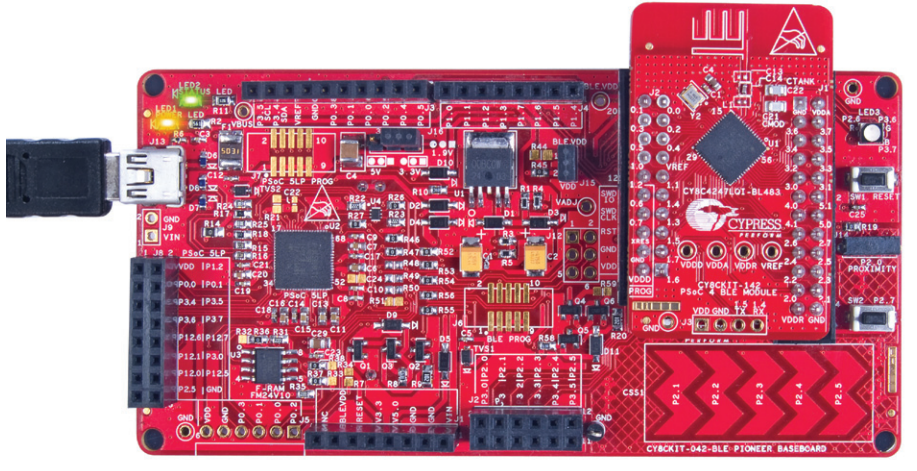
\includegraphics[width=0.5\textwidth]{figures/CY8CKIT-042.png}
\caption{CY8CKIT-042 BLE Pioneer baseboard, samt CY8CKIT-142 PSoC 4 BLE modulet \citep{cypresspsoc2015}.}
\label{fig:CY8CKIT-042}
\end{figure}

I \autoref{fig:CY8CKIT-042}, ses de valgte komponenter, der består af et CY8CKIT-042 BLE Pioneer baseboard og et CY8CKIT-142 PSoC 4 BLE modul. Baseboardet er platformen, hvorpå sensorerne vil blive tilkoblet, og konvertere de analoge signaler til digitale signaler.\fxnote{menes der her, at sensorerne konverterer signalet, eller at det sker på baseboardet - uklart?} Baseboardet har mulighed for tilkobling af en spændingsforsyning, bestående af et $3~V$ knapcelle batteri, eller via mikro USB tilslutningen \citep{cypressguide2014}. Der er mulighed for udvidelse af baseboardet, ved anvendelse af moduler fra Cypress, samt Arduino shields eller 6-pins Digilent Pmod udvidelseskort \citep{cypressguide2014}. 
\\

For at kunne kommunikere trådløst benyttes CY8CKIT-142 PSoC 4 BLE, der et Cypress BLE modul. Kommunikationstypen er Bluetooth Low Energy (BLE) også kendt som Bluetooth SMART \fxnote{relevans? + tilføj noget om, hvad BLE er}, der har en operationsfrekvens på $2,4~GHz$ \citep{cypressguide2014}. 
\\

Ud over de to mikrocontrollere til det endelige system, benyttes en BLE-dongle, der giver mulighed for at en computer kan kommunikere trådløst med systemet. Dette tillader således trådløs test og debugging af systemet. BLE-donglen forsynes via USB-porten på den givne computer med $5~V$ \citep{cypressguide2014}. 
\\

Til at programmere og debugge mikrokontrollerne, benyttes det tilhørende Cypress software, PSoC Creator 3.3. 

%Systemet vil består af et baseboard, hvortil signalet fra de forskellige sensorer vil blive tilsluttet. De anvendte sensorer i dette system kan læses i afsnit ??. Systemet har yderligere mulighed for at blive udvidet med arduinu shields og 6-pins Digilent Pmod udvidelses kort \citep{cypressguide2014}. Baseboardet kan forsynes via et 3 V kanpcelle batteri, eller via USB forbindelse. 

%OPerationsspændinger 1,9 V, 3 V, 3,3 V, eller 5 V \citep{cypress2014}. 
%En enhed der benyttes i systemet er Baseboard'et er den primære komponent i dette system, da denne er ansvarlig for databehandling. Baseboard'et kan tilsluttes andre moduler fra Cypress, samt komponenter som for eksempel arduino shields og 6-pins Digilent Pmod udvidelses kort \citep{cypress2014}. Yderligere vil diverse sensorer, anvendt i systemet, blive tilsluttet til baseboard'et, hvortil vil ske en analog-digital konvertering af signalet. Strømforsyningen til baseboard'et består af et 9 V knapcelle batteri, eller ved tilslutning af USB forbindelse.  

%I dette projekt vil baseboardet blive suppleret med et CY8CKIT-142 PSoC \fixme{PSoC: Programmable System-on-Chip} 4 BLE modul til formål at tillade trådløs kommunikation. Kommunikationens typen kaldes for Bluetooth SMART også kendt som Bluetooth Low Energy (BLE) \citep{cypressguide2014}.
%2,4 GHz radio.


%BLE dongle kan tilsluttes en computer, og har en PRoC BLE enhed til kommunikation. Forsynes med 5 V via USB. Dette tilader computeren at kommunikere med systemet, og at teste og debugge systemet.

%Programmerings- og debug værktøjet til det valgte hardware er PSoC Creator 3.3